\chapter{Experiments}
\label{chapter5}
We evaluated the performance of our agents within a range of domains, from self-designed domains to classic-control tasks. Most experiments were performed using OpenAI Gym \cite{1606.01540} and Behaviour Suite \cite{osband2020bsuite}. We organise the experiments into those that took place within deteriministic domains, and those which took place in stochastic domains. As baselines for evaluation, we used the PRL agent and $\epsilon$-greedy described in Chapter \ref{chapter2}. We chose the PRL agent, because we wanted to compare against a naive model-based exploration approach. Furthermore, we chose $\epsilon$-greedy as we wanted to compare to the most ubiquitous random exploration approach.
\section{Deterministic Domains}
\subsection{Gridworld}
A deterministic gridworld, where the agent begins in the bottom middle, and needs to navigate to the goal state, using the actions "up", "down", "left" and "right". There is an open door, that if closed the agent wouldn't know how to open. All transitions return a reward of -1. The model that the model-based agents were seeded with indicated that the door was closed.

\begin{figure}[H]
    \centering
    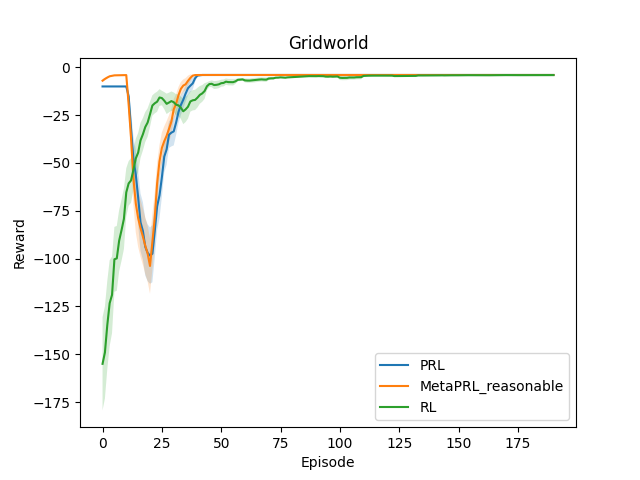
\includegraphics[max size={250}{250}]{report/assets/gridworld.png}
    \caption{Gridworld Results}
    \label{fig:deterministic_gridworld}
\end{figure}

\begin{table}[h]
\centering
\begin{tabular}{|c|c|c|c|c|c|}
\hline
\textbf{Agent} & \textbf{Min} & \textbf{Max} & \textbf{Mean} & \textbf{Std. Dev} & \textbf{Final}\\ \hline
\textbf{MetaPRL} & -104 & -4 & -10 & 19 & -4\\ \hline
\textbf{PRL} & -102 & -4 & -11 & 20 & -4\\ \hline
\textbf{RL} & -168 & -4 & -15 & 28 & -4 \\ \hline
\end{tabular}
\caption{Reward Summary for Gridworld}
\label{tab:example_table}
\end{table}




\subsection{Cliff-Walking}
The Cliff-Walking domain \cite{Sutton1998} is a deterministic gridworld, where the agent begins in the bottom left corner and needs to navigate to the goal state in the bottom right corner by using the actions "up", "down", "left" and "right". However, there is a cliff along the bottom of the grid. The goal of the agent is to reach the goal state whilst avoiding the cliff, as stepping into the cliff returns the agent to the start state (without ending the episode) and induces a large reward penalty of -100. All other transitions return a reward of -1. The model that the model-based agents were seeded with indicated that the cliff was bigger than it actually is; the cliff in the model took up the bottom two rows (minus the end states).

% This domain can be seen in Figure \ref{fig:cliff_walking}.

\begin{figure}[H]
    \centering
    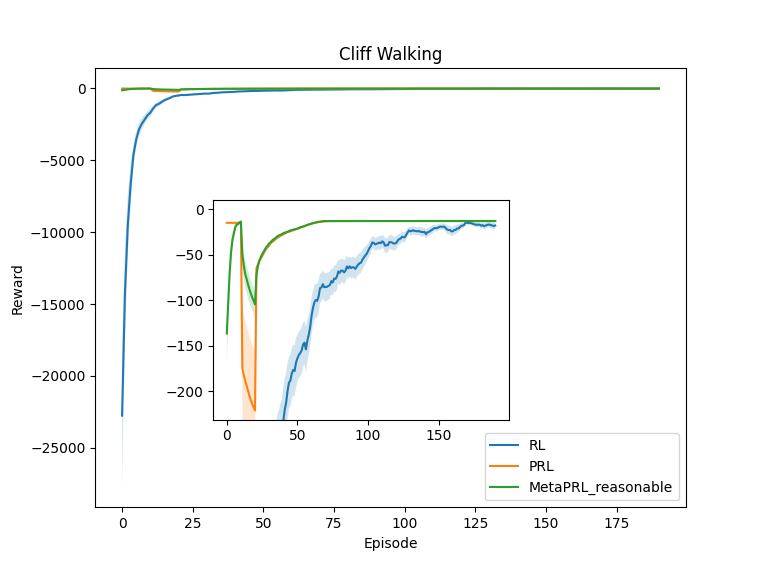
\includegraphics[max size={250}{250}]{report/assets/cliff_walking.png}
    \caption{Cliff-Walking Results}
    \label{fig:cliff_walking}
\end{figure}

\begin{table}[h]
\centering
\begin{tabular}{|c|c|c|c|c|c|}
\hline
\textbf{Agent} & \textbf{Min} & \textbf{Max} & \textbf{Mean} & \textbf{Std. Dev} & \textbf{Final}\\ \hline
\textbf{MetaPRL} & -137 & -13 & -22 & 21 & -13\\ \hline
\textbf{PRL} & -221 & -13 & -27 & 42 & -13\\ \hline
\textbf{RL} & -23099 & -14 & -520 & 2228 & -14 \\ \hline
\end{tabular}
\caption{Reward Summary for Cliff-Walking}
\label{tab:example_table}
\end{table}

\subsection{Windy Gridworld}
\label{sec:windy}
The Windy Gridworld domain \cite{Sutton1998} is a deterministic gridworld, where the agent most navigate from the start state to the goal state, by using the actions "up", "down", "left" and "right". However, there is "wind" through the middle of the grid which varies in strength. The wind shifts the next state upwards by the strength of the wind. All transitions return a reward of -1. The model that the model-based agents were seeded with did not model the wind; thus the agents were unaware of it.

\begin{figure}[H]
    \centering
    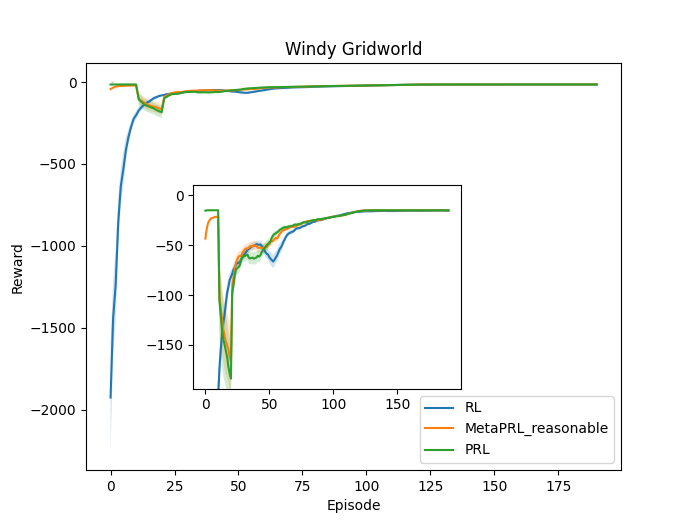
\includegraphics[max size={250}{250}]{report/assets/windy.png}
    \caption{Windy Gridworld Results}
    \label{fig:deterministic_wind}
\end{figure}

\begin{table}[h]
\centering
\begin{tabular}{|c|c|c|c|c|c|}
\hline
\textbf{Agent} & \textbf{Min} & \textbf{Max} & \textbf{Mean} & \textbf{Std. Dev} & \textbf{Final}\\ \hline
\textbf{MetaPRL} & -168 & -15 & -33 & 30 & -15\\ \hline
\textbf{PRL} & -183 & -15 & -34 & 33 & -15\\ \hline
\textbf{RL} & -2061 & -15 & -74 & 216 & -15 \\ \hline
\end{tabular}
\caption{Reward Summary for Windy Gridworld}
\label{tab:example_table}
\end{table}

% This domain can be seen in Figure \ref{fig:cliff_walking}.

% \begin{figure}[h!]
%     \centering
%     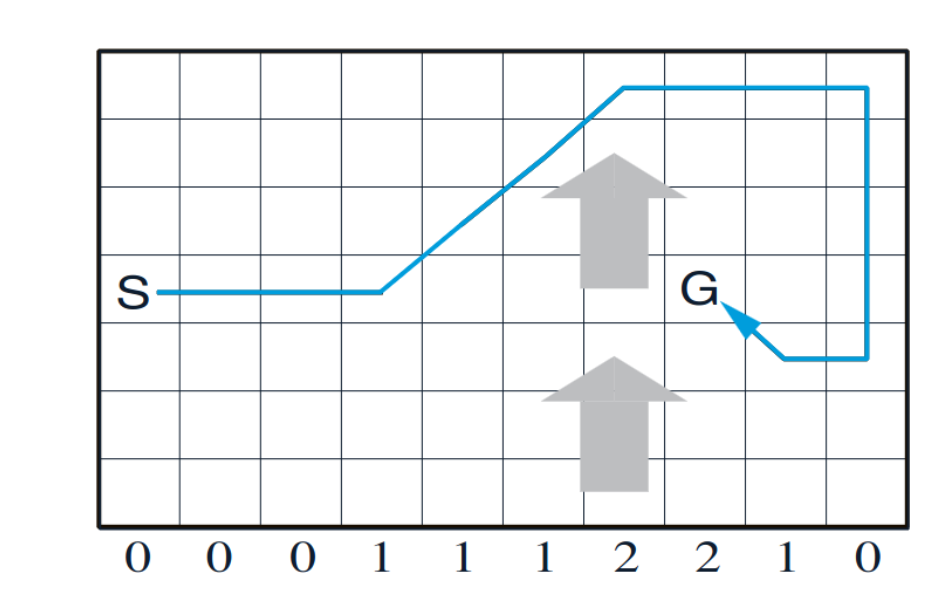
\includegraphics[max size={200}{200}]{report/assets/envs/windy.png}
%     \caption{Windy Gridworld}
%     \label{fig:deterministic_wind}
% \end{figure}


% \subsection{Cart-Pole}
% The Cart-Pole domain \cite{1606.01540, 6313077} consists of a pole placed on top of a moving cart, with the goal being to balance the pole by applying forces to the cart. There are two actions available to the agent; push cart left and push cart right. The agent's state is described by four variables; the cart's position, the cart's velocity, the pole's angle and the pole's angular velocity. 

% \begin{figure}[h!]
%     \centering
%     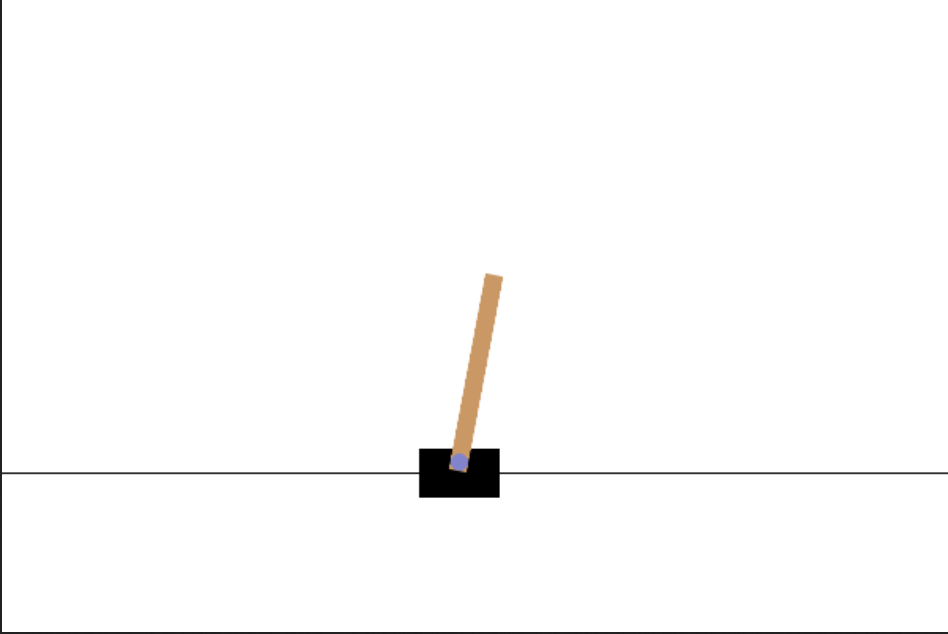
\includegraphics[max size={200}{200}]{report/assets/envs/cartpole.png}
%     \caption{Cartpole}
%     \label{fig:cartpole}
% \end{figure}


% \subsection{Mountain Car}
% The Mountain Car domain consists of a car placed stochastically in between two mountains, with the goal of getting to the top of the hill \cite{1606.01540, Moore90efficientmemory-based}. There are three actions available to the agent; accelerate left, don't accelerate and accelerate right. The agents state is described by two variables; it's velocity and it's position along the x-axis. 
% The transition function can be described by the following equations:
% \begin{equation}
% \label{eqn:mcdnl}
% \text{velocity}_{t+1} = \text{velocity}_t + (D * \text{F}) - \cos{(3*\text{position}_t)} * g
% \end{equation}
% \begin{equation}
% \label{eqn:mcdnr}
% \text{position}_{t+1} = \text{position}_t + \text{velocity}_{t+1}
% \end{equation}
% Where $D$ is the direction of acceleration: left = -1, none = 0, right = +1.
% All transitions return a reward of -1 and episodes are terminated after 200 time steps, if the goal has not been reached.


% \begin{figure}[h!]
%     \centering
%     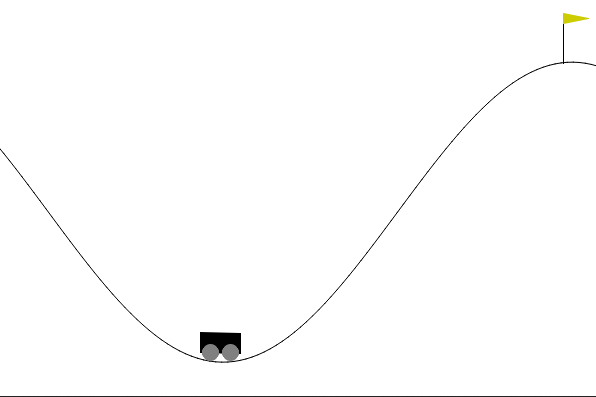
\includegraphics[max size={200}{200}]{report/assets/envs/mountaincar.png}
%     \caption{Mountain Car}
%     \label{fig:mountaincar}
% \end{figure}


\section{Stochastic Domains}


\subsection{Stochastic Gridworld}
A simple gridworld, with a door that is open with probability 0.5, closed otherwise. The model embedded suggests that the door is closed with probability 1.0.

A stochastic gridworld, where the agent begins in the bottom middle, and needs to navigate to the goal state, using the actions "up", "down", "left" and "right". The door is open with probability 0.6 and closed otherwise. The agent does not have the ability to open the door. All transitions return a reward of -1. The model that the model-based agents were seeded with indicated that the door was closed with probability 1.0.

\subsection{Stochastic Windy Gridworld}
This is a stochastic version of the Windy Gridworld described in Section \ref{sec:windy}. The modification that makes it stochastic is that the wind (if there is any) is stochastic. Apart from that, the general setup is the same as previously described. Similarly, the model that the model-based agents were seeded with did not model the wind; thus the agents were unaware of it.

%and seen in Figure \ref{fig:deterministic_wind}.

\subsection{Frozen Lake}
The Frozen Lake domain \cite{1606.01540} is a stochastic gridworld, where the agent must navigate from the start state in the top left corner to the goal state in the bottom right corner, by using the actions "up", "down", "left" and "right". However, the frozen lake is slippery, meaning that the agent moves in the intended direction with probability $\frac{1}{3}$ and in either of the perpendicular directions with probability $\frac{1}{3}$ each. Furthermore, there are holes where the ice has been broken or melted and entering these holes end the epsisode. Rewards are sparse; reaching the goal state returns a reward of +1, whilst all other transitions return a reward of 0. The model that the model-based agents were seeded with did not model the slippery nature of the lake; thus the agents were unaware of it.

\section{An Ablation Study: Learning from Scratch}
Within Chapter \ref{chapter2}, we stated that learning from scratch is a weakness of other model-based exploration approaches as models created by humans can be useful for learning. However, an interesting question is: is the usefulness of models created by humans worth the time it takes to construct them? This is what we investigate in this section. We seeded the various agents with optimistic initial models, as in the approach followed by R-MAX and OIM, however the so-called "Garden of Eden State" was a real-state in the environments, namely the actual goal state. Hence, the model suggests that every transition leads to the goal state.
% \section{Results}


% % This domain can be seen in Figure \ref{fig:frozen}

% \begin{figure}[h!]
%     \centering
%     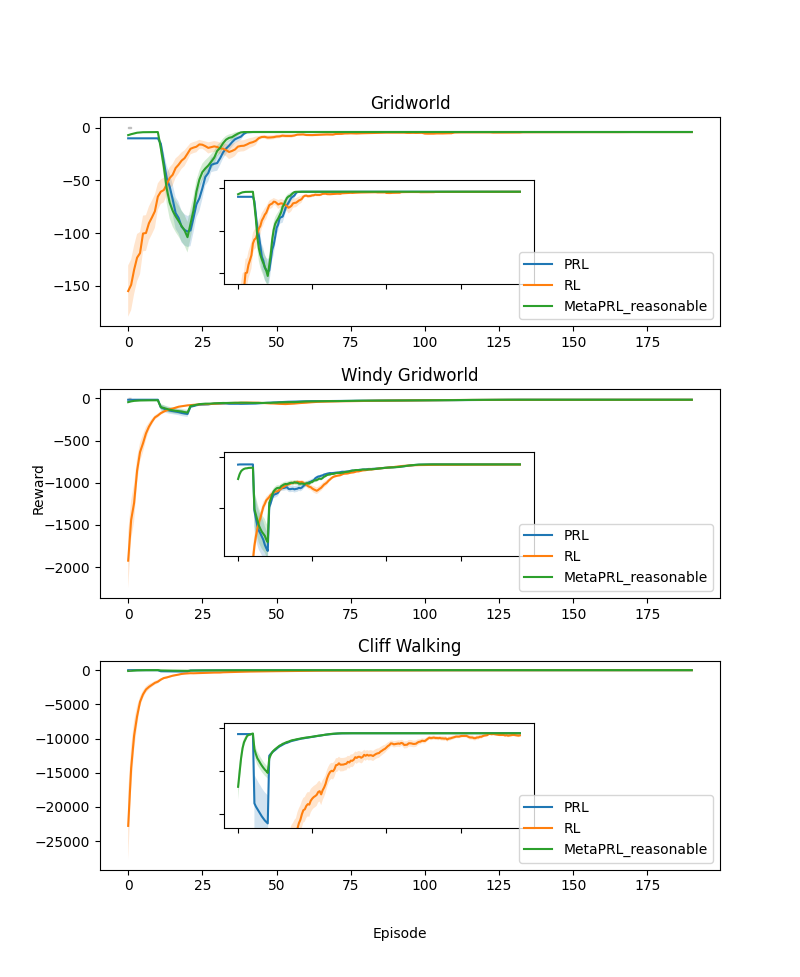
\includegraphics[max size={500}{500}]{report/assets/results.png}
%     \caption{Deterministic Results}
%     \label{fig:deterministic_results}
% \end{figure}